\chapter{Présentation du matériel}

\section{La \textit{RaspberryPi}}

Si vous avez été intriguer par la bête que je vous ai mis en photo dans l'introduction, pas de panique, elle va devenir votre nouvelle meilleure amie. Il s'agit ni plus ni moins que d'un ordinateur en modèle réduit.
Cette puce est capable de faire tourner une distribution de \textit{Linux} connue sous le nom de \textit{Raspbian}. La \textit{RaspberryPi} est un véritable bijoux de miniaturisation pour les \textit{Makers} qui désire embarquer des ordinateurs dans leur projets les plus fou. Vous l'aurez compris, cela va être notre base de notre station.\\

\textit{Pourquoi ce choix ? }\\

La \textit{RaspberryPi} peut être repoussante au début car vendue tel que vous avez pu la voir  plus tôt mais une fois prise en main, elle est simple d'utilisation. Elle permet d'avoir un accès internet de façon simple avec son port ethernet, on peut y brancher un écran ainsi que des périphériques si nécessaire pour réaliser de la maintenance (même si il existe d'autre moyen d'y accéder mais nous verrons ça plus tard). 
Une raison non négligeable pour notre projet est son prix. Compté une quarantaine d'euros pour le dernier modèle en date.
Elle possède également des broches pour réaliser de l'électronique embarquée comme nous allons le faire. Ainsi notre ordinateur est modulaire et on peut y ajouter des composants par ces broches.\\

\begin{figure}[H]
\begin{center}
	\makebox[\textwidth]{\includegraphics[width=.7\paperwidth]{images/pinrpi.png}}
\end{center}
	\caption{ \textit{Pin Mapping de la RaspberryPi 3}}
\end{figure}\\

Son autre atout et non des moindre, c'est sa communauté qui s'est étendue de façon exponentielle ces dernières années car accessible à tout le monde et permet alors une aide conséquente via les forums.

Vous voilà plus familier avec l'engin, si vous voulez plus d'information, je vous laisse visiter \href{https://www.raspberrypi.org/}{le site officiel} où vous pouvez notamment télécharger la version de base de son OS, \textit{Raspbian} mais qui possède nombre de version modifié (un OS pour réaliser une station de jeux rétro est un exemple)

\section{Le shield \textit{GrovePi+}}

Je vous parlait juste avant que la \textit{RaspeberryPi} possédait des broches. Ces dernière vont nous servir à y installer les capteurs. Mais nous n'allons pas brancher les capteurs directement sur la \textit{RaspberryPi}. En effet nous allons ajouter ce que l'on appelle un \textit{"Shield}. Il s'agit ni plus ni moins que d'une autre carte électronique avec ses fonctions propre qui se branche sur la \textit{RaspberryPi} pour communiquer avec elle. Ainsi, nous pouvons utiliser les fonctions du \textit{"Shield"} en envoyant des instruction de puis la \textit{"RaspberryPi}.

Celui que nous utilisons porte le doux nom \textit{GrovePi+}. Sans m'attardez sur ses détails techniques, sachez (pour les connaisseurs) qu'elle embarque un microcontrôleur ATMega pour gérer les capteurs. Il s'agit ni plus ni moins d'une version \textit{"User Friendly"} d'un \textit{Arduino} que l'on branche sur notre \textit{RaspberryPi}.\\

\begin{figure}[H]
\begin{center}
	\makebox[\textwidth]{\includegraphics[width=.7\paperwidth]{images/grovepi.jpg}}
\end{center}
	\caption{ \textit{le Shield GrovePi+}}
\end{figure}\\


Comme vous voyer sur la photo, nous avons des connecteurs \textit{4-pins}, en blanc. C'est là dessus que l'on va brancher nos capteurs.\\
\\
\textbf{ATTENTION : Ces connecteurs sont reliés à des broches particulière du microcontrôleur. Ils sont donc chacun d'entre eux prévu pour un type de composant particulier. } \\

On distingue trois types de connecteurs parmis ceux-là :

\begin{itemize}
	\item ports analogiques : Ils sont disponible uniquement en \textit{INPUT}, c'est à dire qu'il s'agit d'une entrée pour une tension comprise entre 0 et 5V. Le \textit{Shield} possède un convertisseur analogique numérique qui échantillonne cette valeur sur 10bits (0V = 0 et 5V = 1023. Exemple si on envoie 2.5V, alors on aura la valeur 512)
	
	\item ports digitaux : ceux ci peuvent être régler en \textit{INPUT} ou en \textit{OUTPUT}. Comme ce sont des entrée/sortie numérique, elle répond à la loi du tout ou rien. Soit nous avons 0V, soit nous avons 5V (0 ou 1). Typiquement, pour une sortie cela peut être utilisé comme interrupteur électronique.
	\item ports I2C : Il s'agit d'un protocole de communication développé par Philips pour minimiser le nombre de fil nécessaire pour faire communiquer deux périphériques entre eux. Il y a en effet uniquement 3 fils : un signal de données (SDA), un signal d'horloge (SCL), et un signal de référence électrique (masse).
\end{itemize}

Nous allons maintenant parler rapidement des différents capteurs et composants que nous allons brancher sur notre \textit{Shield}

\section{Les composants}

\subsection{Le capteur de température et d'humidité}

Les capteurs d'humidité répondent à une loi qui dépend de la température. C'est pour cette raison que ces capteurs fournissent bien souvent les deux à la fois. De notre côté, il s'agit du capteur \textit{DHT11}. Ce composant utilise un connecteur digital\\

\begin{figure}[H]
\begin{center}
	\makebox[\textwidth]{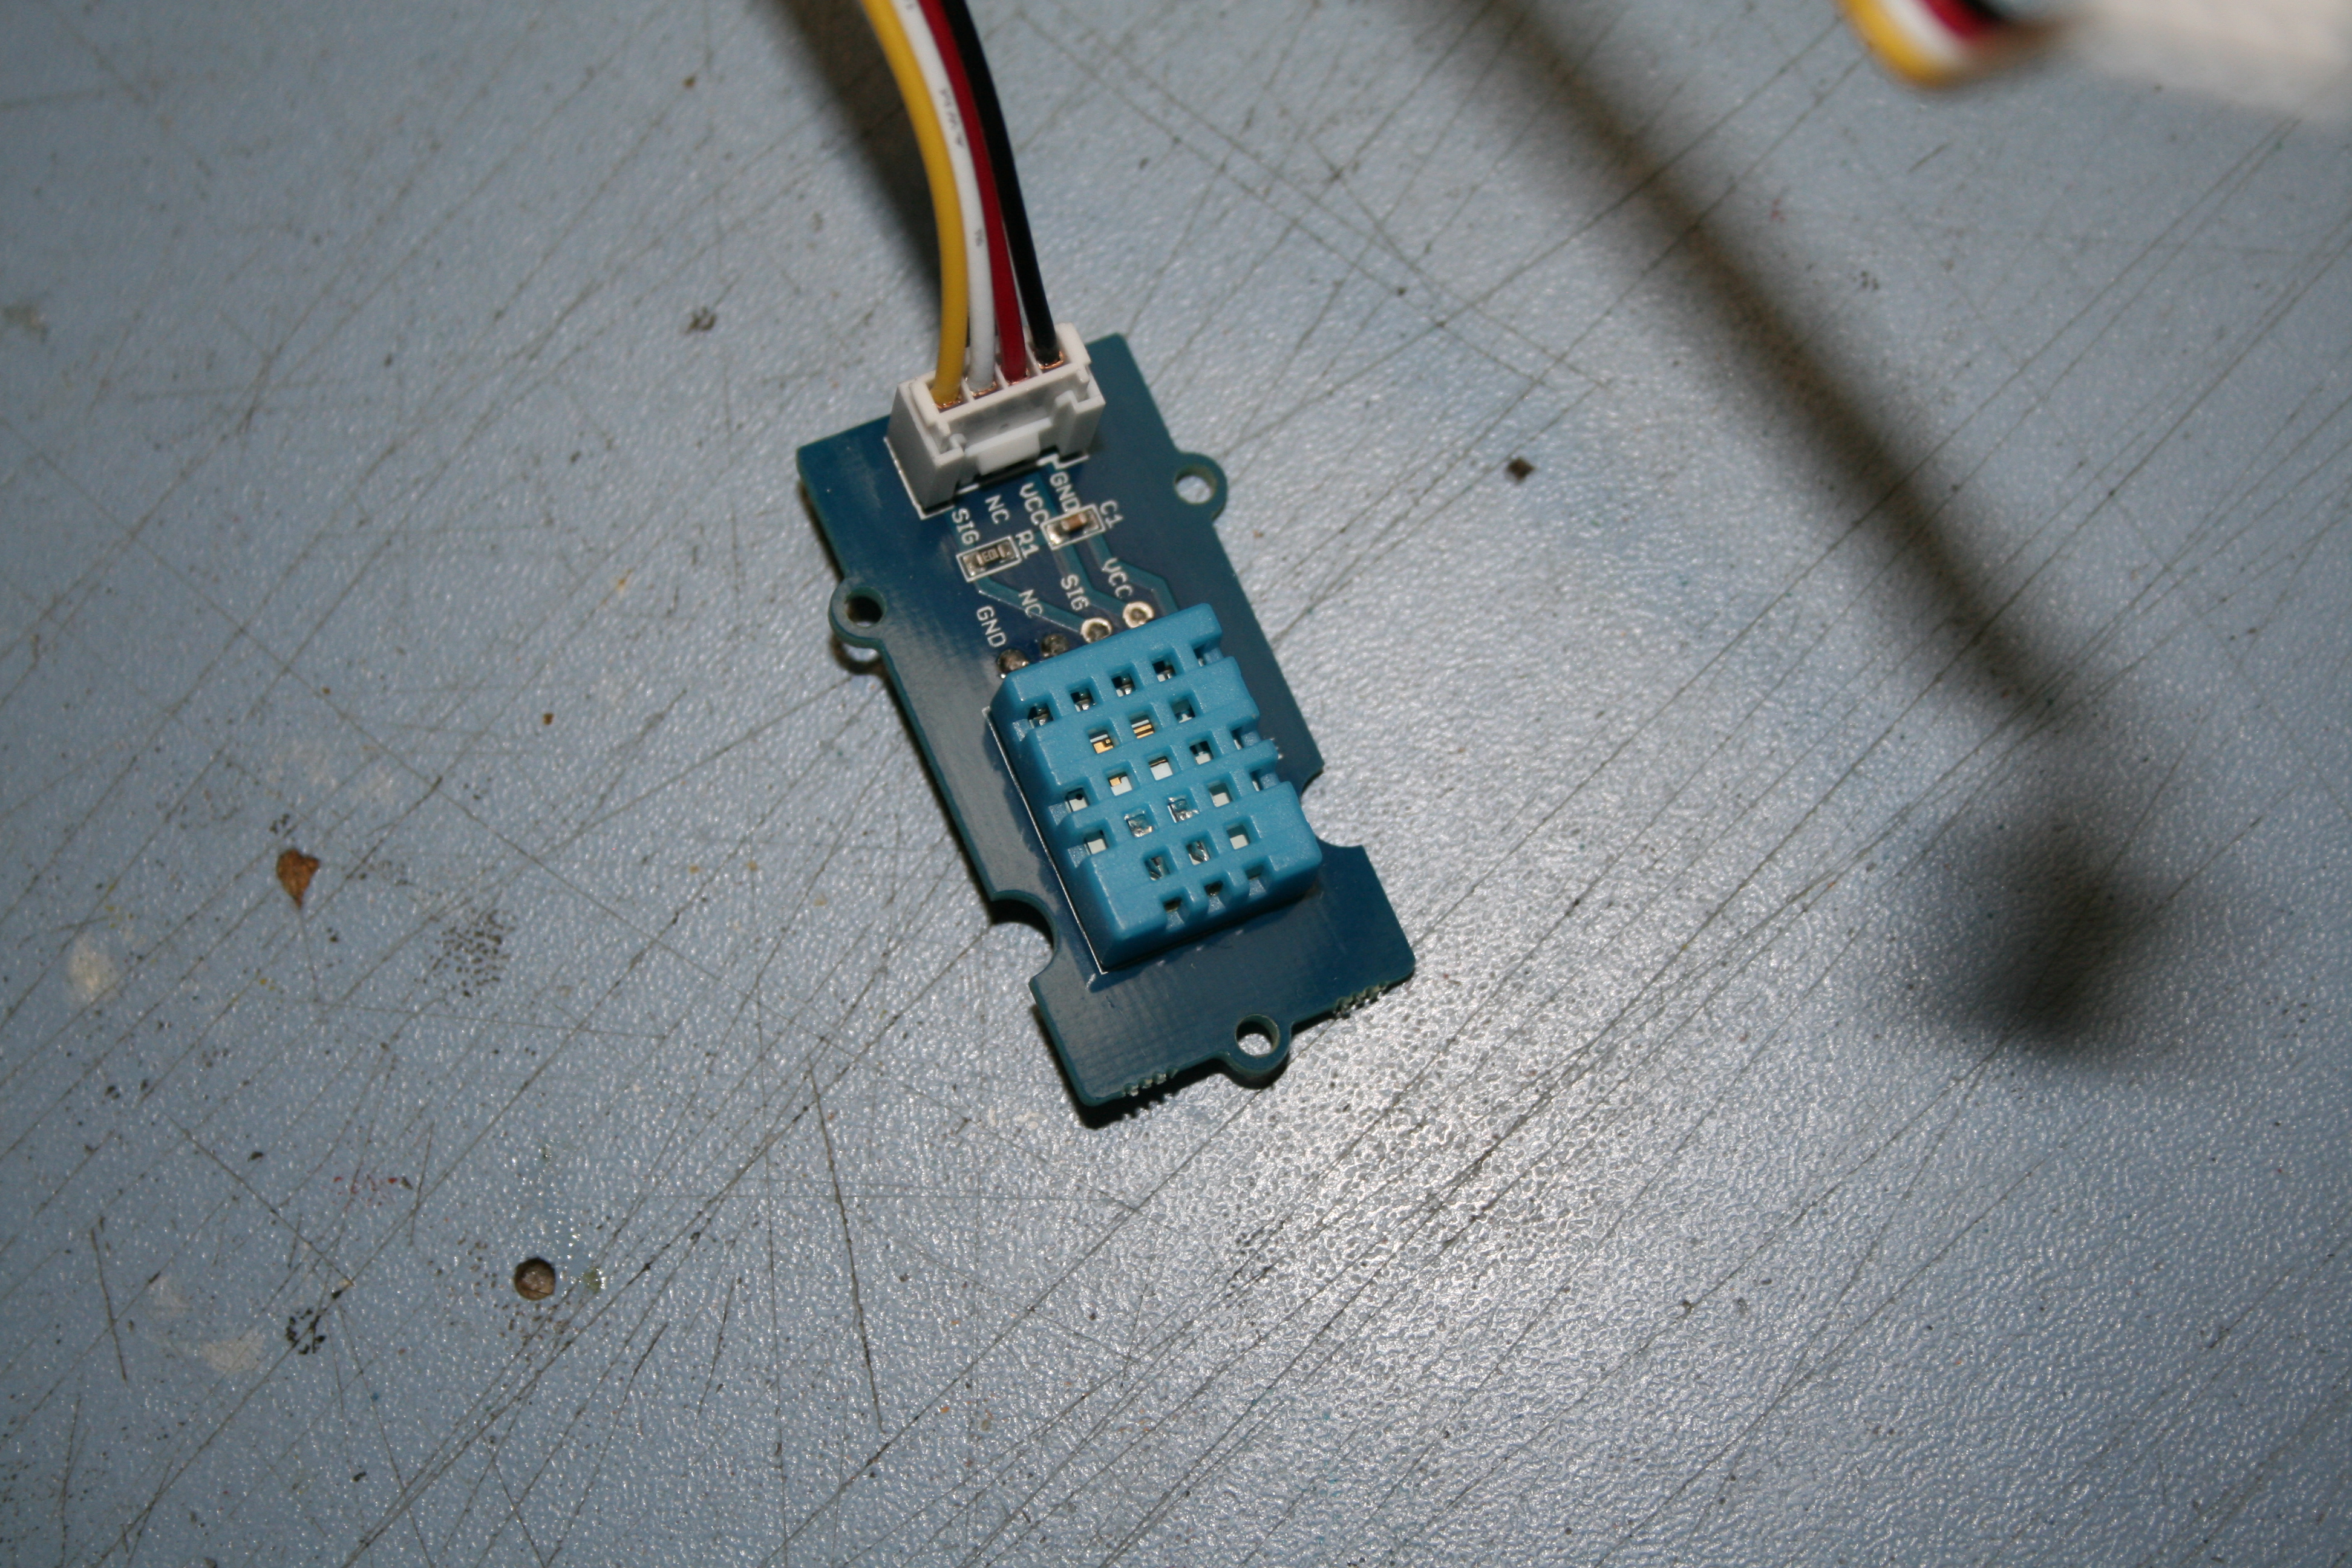
\includegraphics[width=.5\paperwidth]{images/dht11.jpg}}
\end{center}
	\caption{ \textit{Capteur d'humidité et de température}}
\end{figure}\\

\href{https://akizukidenshi.com/download/ds/aosong/DHT11.pdf}{Datasheet du DHT11}

\subsection{Le capteur de luminosité}

Le capteur de luminosité mesure la lumière ambiante. Exprimé en Luxmètre, les capteurs de luminosité "basique" ne permettent pas d'obtenir une valeur précise de la luminosité. Néanmoins, cette valeur est très abstraite pour l'utilisateur. C'est pour cette raison que nous allons l'utiliser pour déterminer si la lumière de la pièce où il est placé est allumé ou non. Nous détaillerons un protocole à réaliser pour essayer de faire marcher au mieux ce capteur. Ce composant utilise un connecteur analogique.\\

\begin{figure}[H]
\begin{center}
	\makebox[\textwidth]{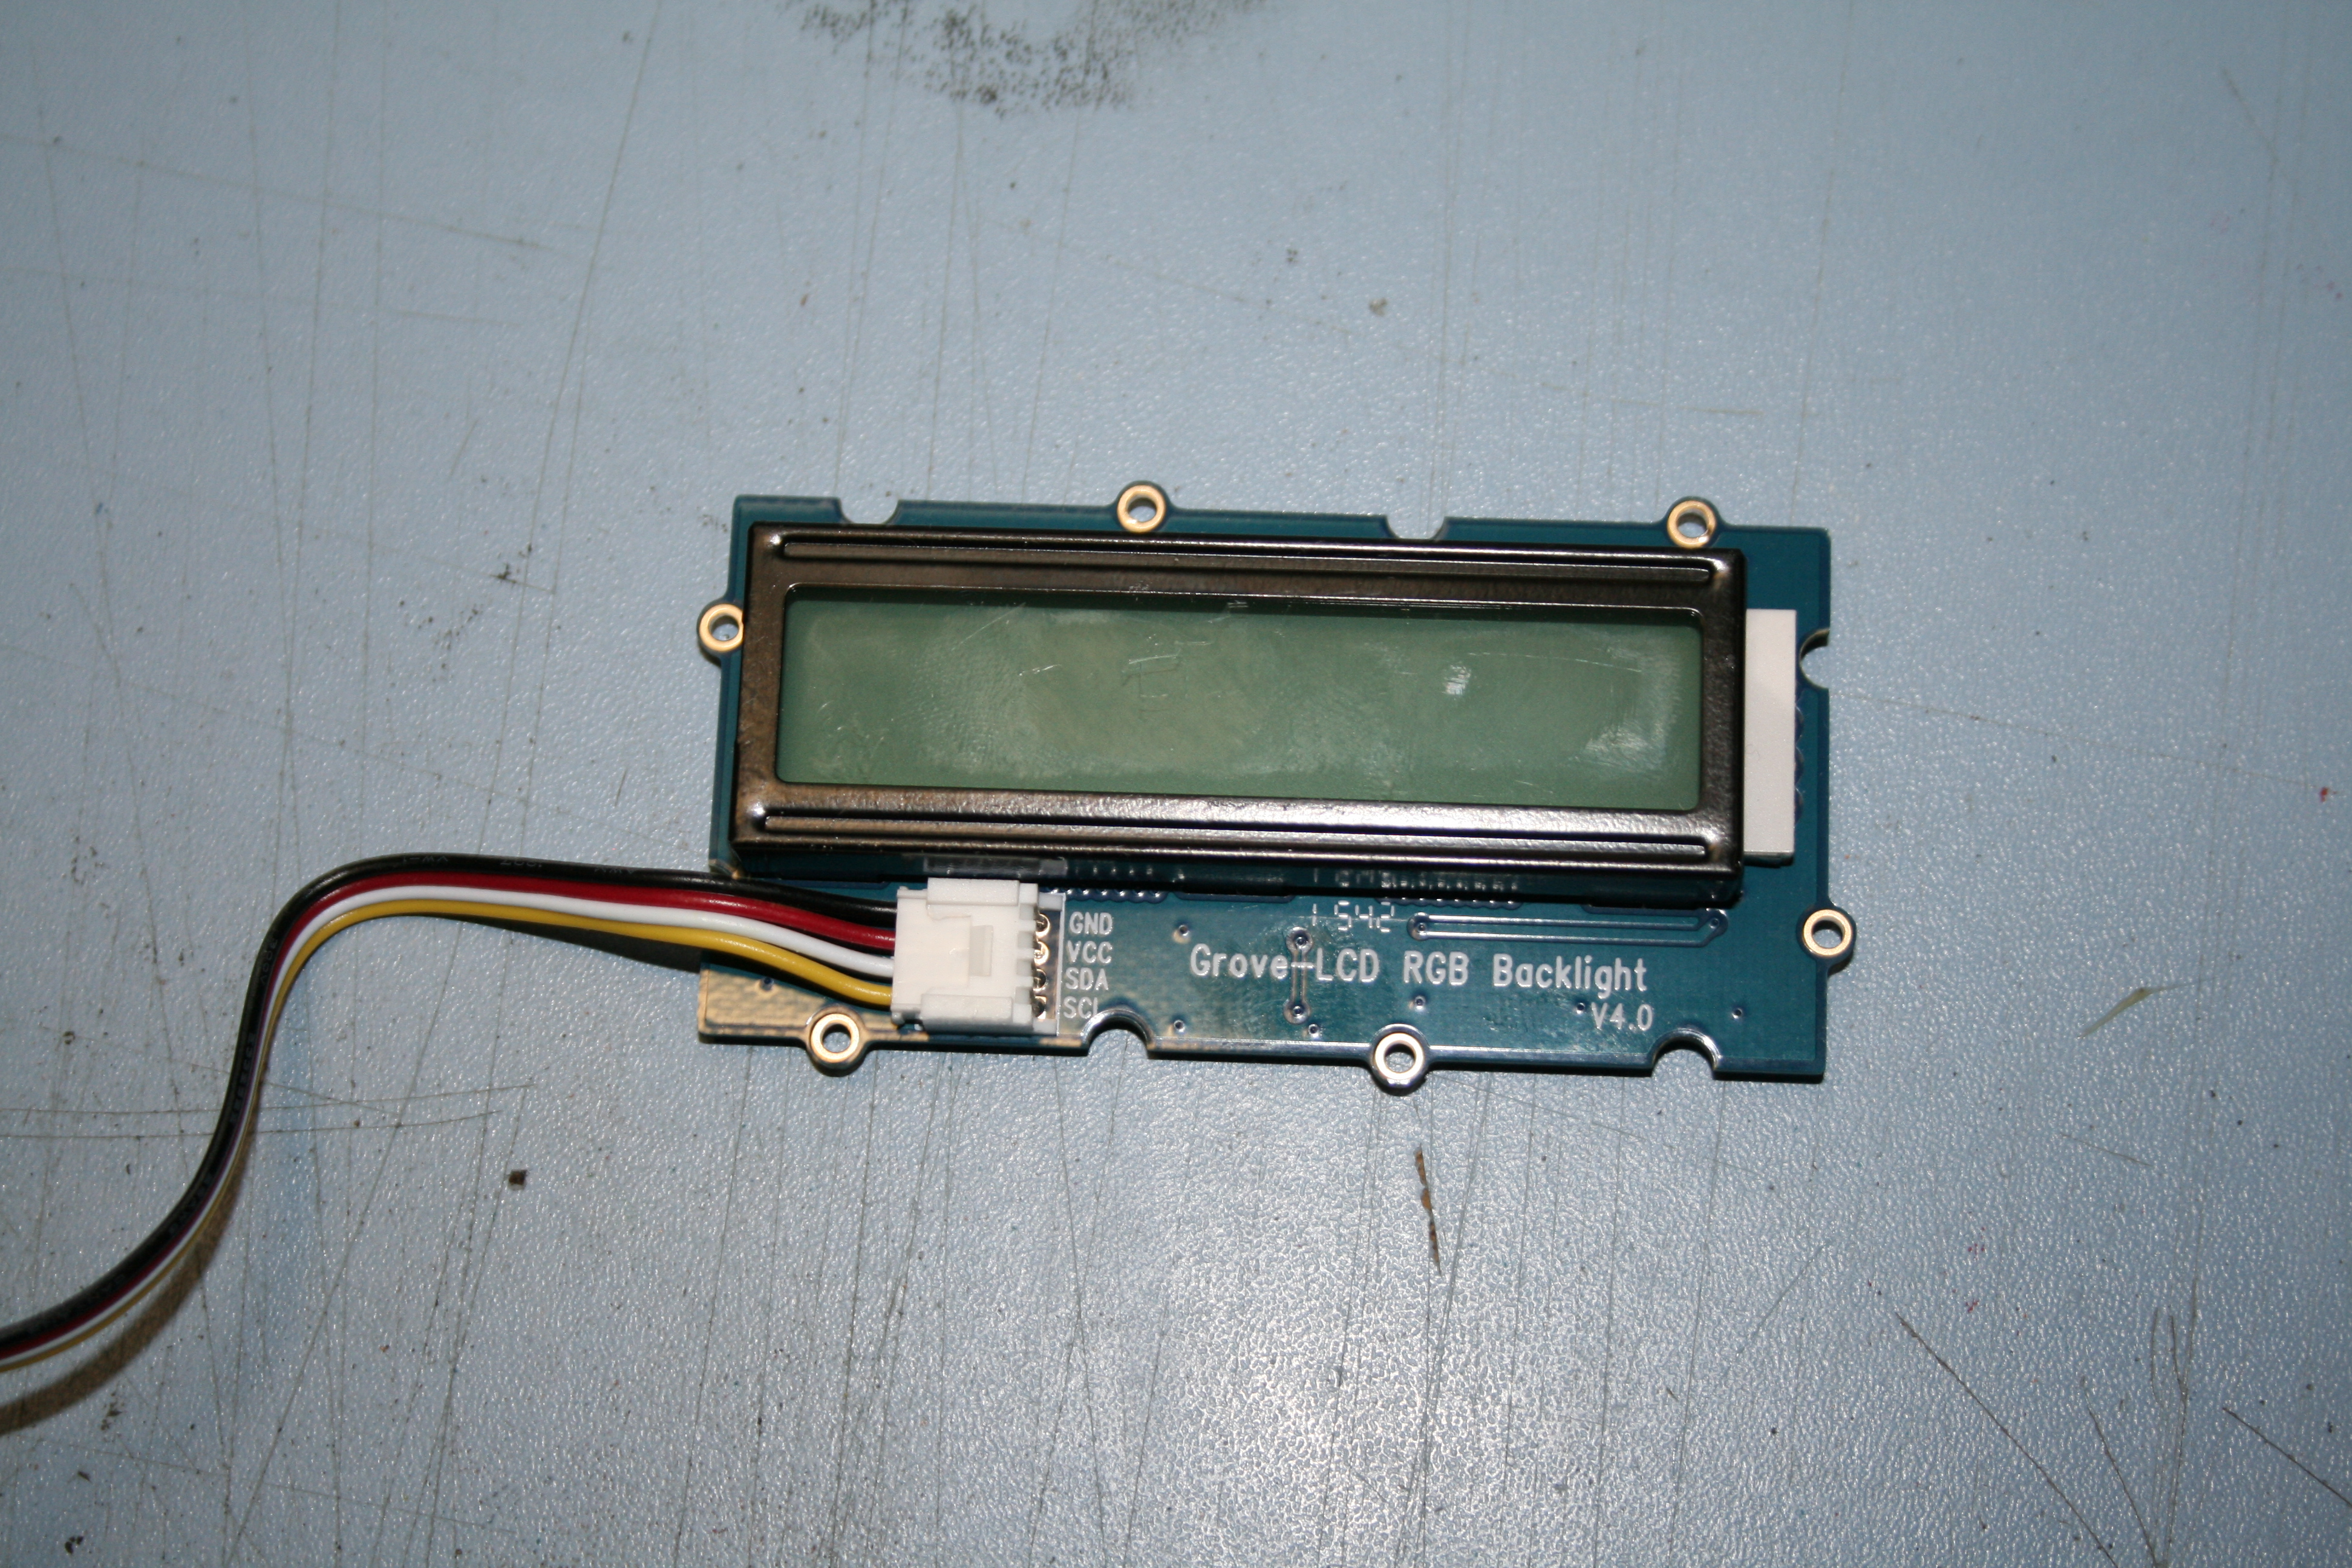
\includegraphics[width=.5\paperwidth]{images/lcd.jpg}}
\end{center}
	\caption{ \textit{L'écran LCD}}
\end{figure}\\

\href{https://github.com/SeeedDocument/Grove_Light_Sensor/raw/master/res/LS06-M%CE%A65_datasheet.pdf}{Datasheet du capteur de luminosité}

\subsection{L'écran}

Pour pouvoir accéder localement aux valeurs des capteurs, nous allons placer un écran.
Nous pouvons afficher 2 lignes de 16 caractère sur ce dernier et choisir la couleur de fond qui est affiché. Ce composant utilise un connecteur I2C.\\

\begin{figure}[H]
\begin{center}
	\makebox[\textwidth]{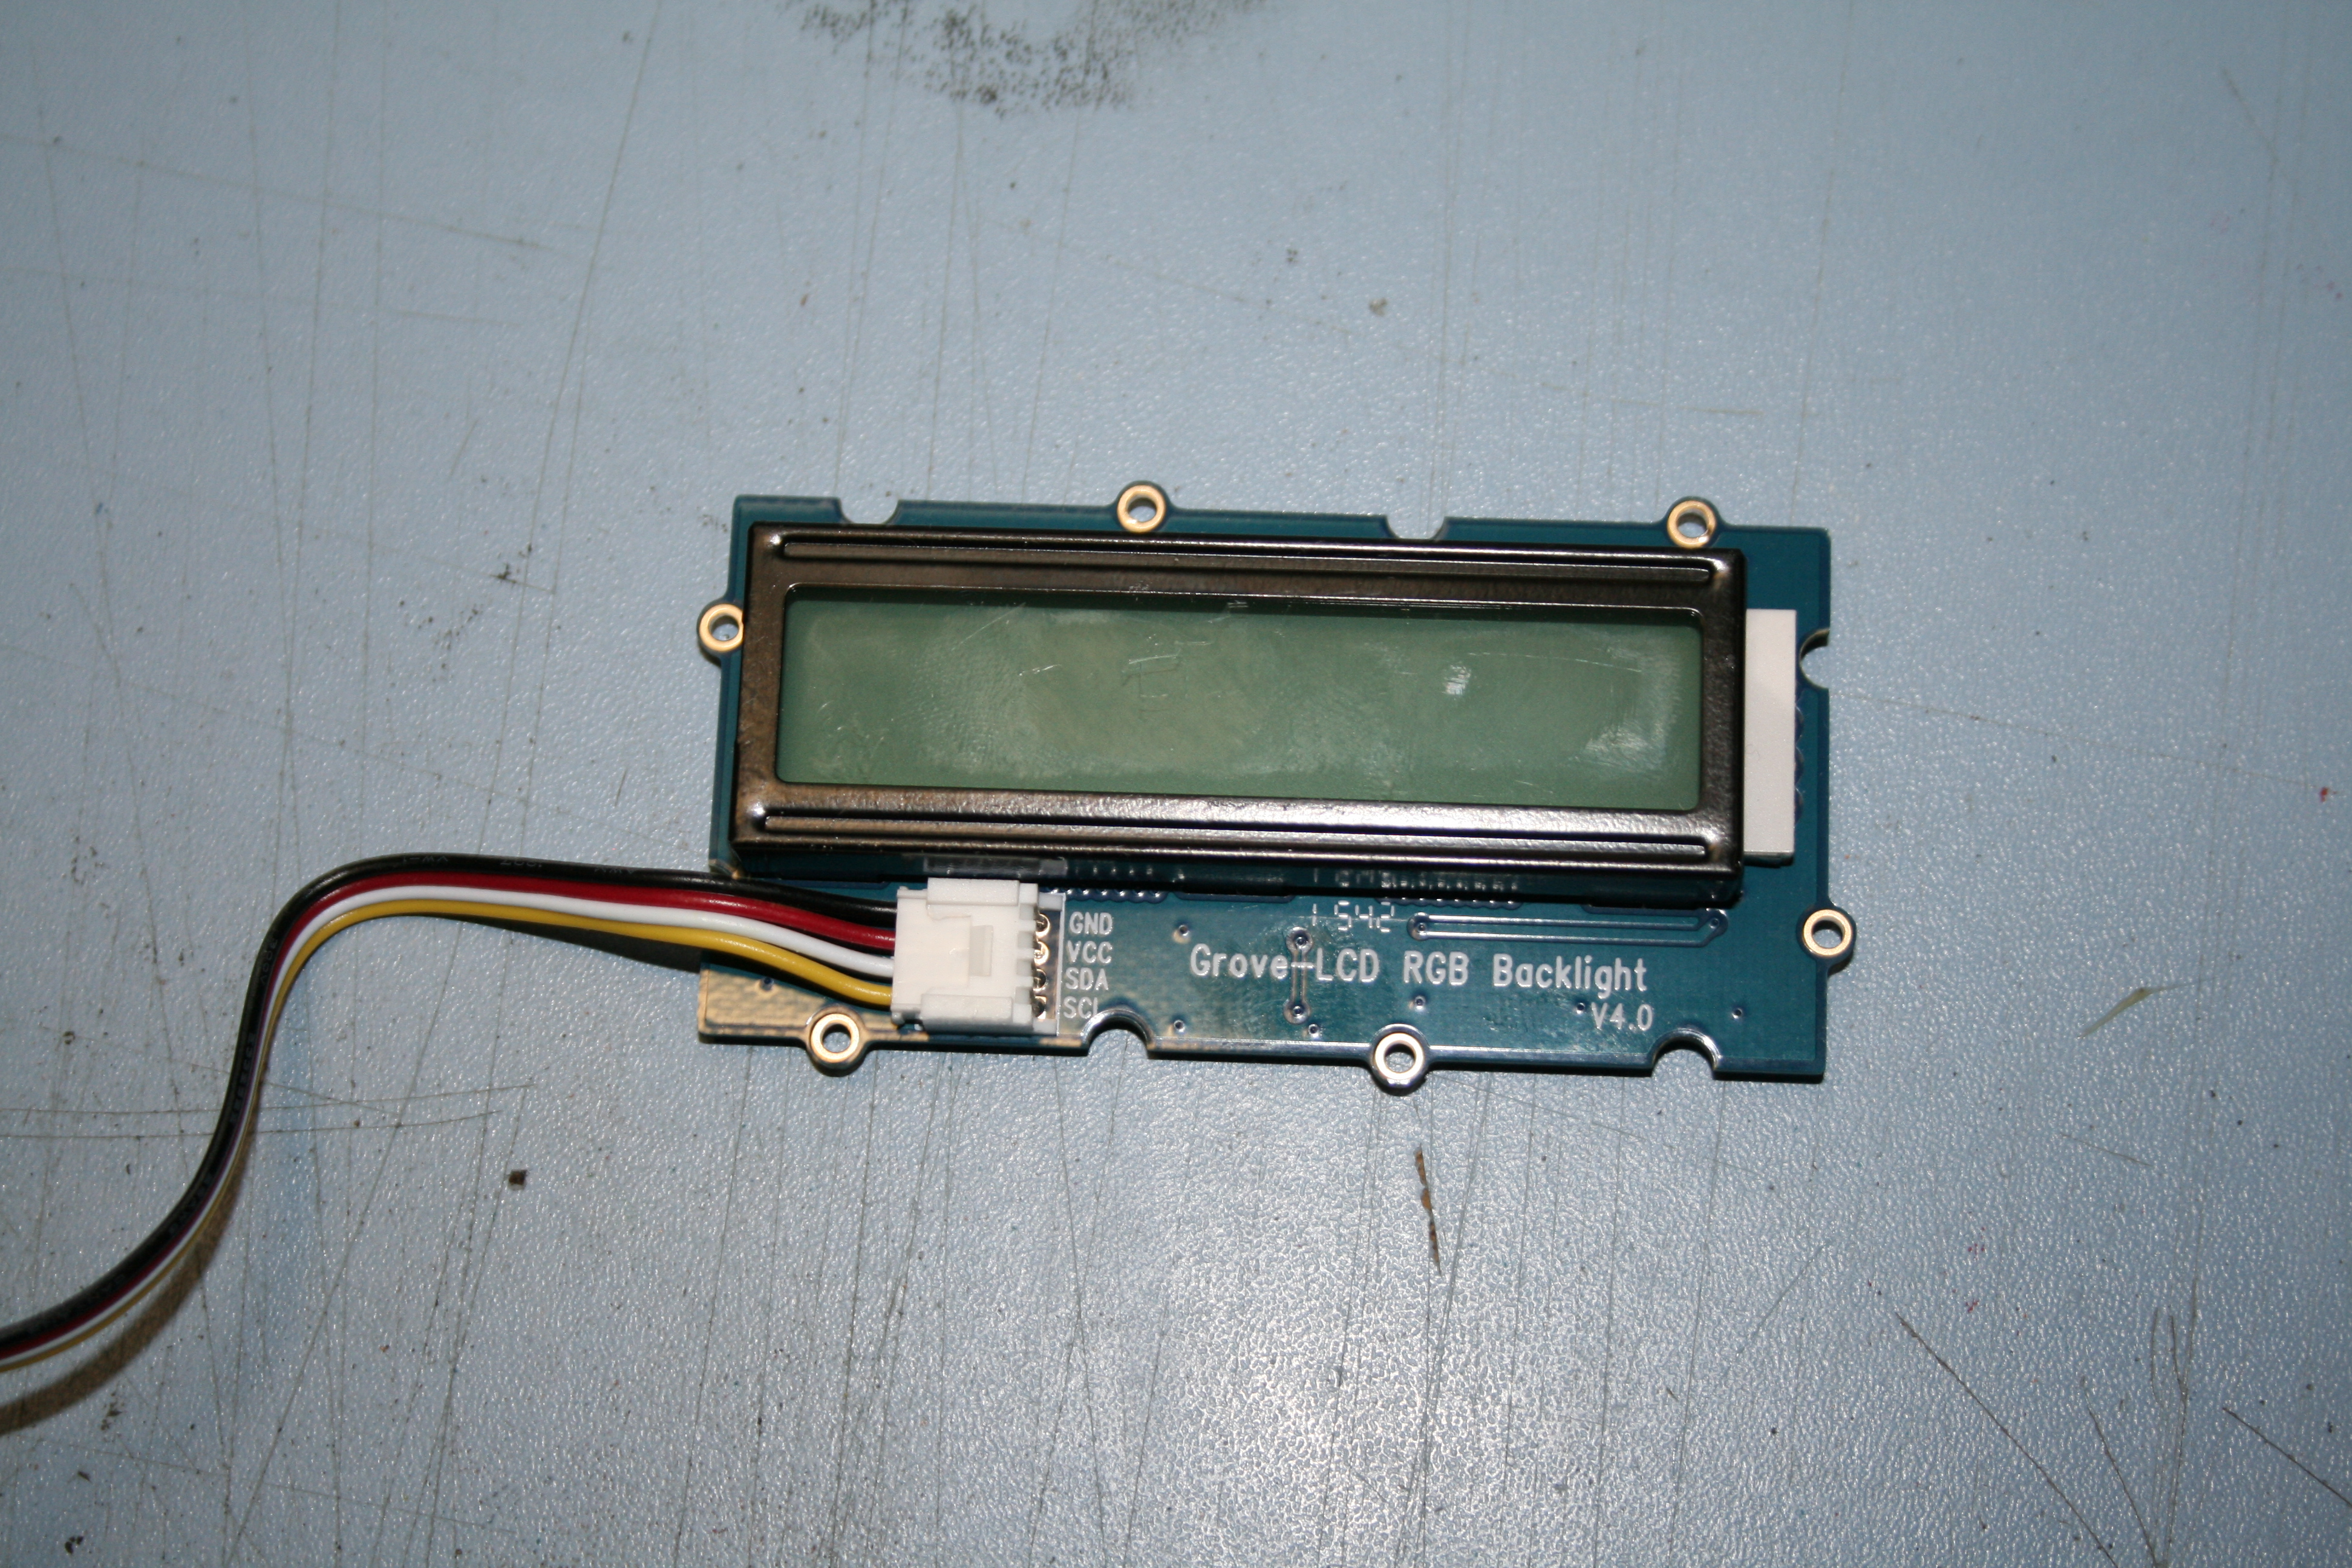
\includegraphics[width=.5\paperwidth]{images/lcd.jpg}}
\end{center}
	\caption{ \textit{L'écran LCD}}
\end{figure}\\

\subsection{L'encodeur rotatif}

Nous n'allons pas l'utiliser comme un capteur à proprement parler ici mais d'un bouton tournant pour naviguer dans différents affichage sur l'écran. On pourra ainsi passer de l'affichage de la température à l'humidité,etc...\\

\begin{figure}[H]
\begin{center}
	\makebox[\textwidth]{\includegraphics[width=.5\paperwidth]{images/encoder.jpg}}
\end{center}
	\caption{ \textit{Encodeur rotatif pour bouton tournant}}
\end{figure}\\

Maintenant que nous avons connaissance du matériel que nous avons à disposition pour notre station, nous allons pouvoir passer à son installation.





